\documentclass[12pt]{article}
\usepackage[utf8]{inputenc}
\usepackage{amsmath}
\usepackage{systeme}
\usepackage{amsfonts}
\usepackage{graphicx}
\usepackage{enumitem}
\usepackage{hyperref}
\usepackage{xcolor}
\usepackage{kbordermatrix}
\usepackage{centernot}
\usepackage{xcolor}

\title{%
	\textbf{Notițe Seminar 7}}

\begin{document}
	
	\maketitle
	
	\textbf{{Intro:}} Seminarul trecut am început să discutăm despre algoritmii Bayes naiv și Bayes corelat. Acum vom continua discuția despre ei cu două mari noi chestiuni:
	\begin{itemize}
		\item 	rata medie a erorilor pentru NB și JB
		\item 	extensia lui NB pentru lucrul cu atribute continue (la intrare)
	\end{itemize}

	\section{Rata medie a erorilor}
	\subsection{Remember 1}
	
	Regulile de decizie finale pentru NB și JB sunt:
	
	$$v_{NB} = \arg \max_{v_j \in V} \underbrace{P(v_j) P(a_1|v_j) \dots P(a_n|v_j)}_{P_{NB}(a_1,\dots,a_n,v_j)}$$
	
	$$v_{JB} = \arg \max_{v_j \in V} \underbrace{P(v_j) P(a_1,\dots,a_n|v_j)}_{P_{JB}(a_1,\dots,a_n,v_j) = P(a_1,\dots,a_n,v_j)}$$
	
	Notația $P_{NB}$ indică faptul că NB folosește distribuția de probabilitate în care folosim presupunerea de independență condițională a atributelor de intrare față de ieșire.
	
	Faptul că $P_{JB} = P$ ($P$ - distribuția reală de probabilitate) nu ar trebui să fie o surpriză, pentru că JB nu face nicio presupunere neconformă cu realitatea.
	
	\subsection{Remember 2}
	$$E[X] = \sum_{x \in X} x P(X = x)$$
	$$E[f(X)] = \sum_{x \in X} f(x) P(X = x)$$
	$$E[XY] = \sum_{x \in X, y\in Y} xy P(X = x, Y = y)$$
	$$E[f(X,Y)] = \sum_{x \in X, y\in Y} f(x,y) P(X = x, Y = y)$$
	
	\subsection{Remember 3}
	Funcția \textbf{indicator}: $I : \{\text{True},\text{False}\} \rightarrow \{0,1\}$, $I(\text{True}) = 1$, $I(\text{False}) = 0$.
	
	\subsection{Rata medie a erorilor: $E_P [{I(v_{NB/JB}(A_1,\dots,A_n) \neq V)}]$}
	
	$$E_{\underbrace{{P}}_\text{distribuția reală}} [\underbrace{I(v_{NB/JB}(A_1,\dots,A_n) \neq V)}_{f(A_1,\dots,A_n,V)}] \stackrel{\text{def.}}{=} $$
	$$ \stackrel{\text{def.}}{=} \sum_{a_1\in A_1,\dots,a_n \in A_n, v_j \in V} \underbrace{I(v_{NB/JB}(A_1=a_1,\dots,A_n=a_n) \neq v_j)}_{f(a_1,\dots,a_n,v_j)} \underbrace{P(A_1=a_1,\dots,A_n=a_n,V=v_j)}_{\text{distribuția reală}} $$
	
	Exercițiu: vezi ex. 28/pag. 414. Vezi rezolvarea din slide-uri: \url{https://profs.info.uaic.ro/~ciortuz/ML.ex-book/SLIDES/ML.ex-book.SLIDES.Bayes.pdf} (începând cu slide-ul \#48).
	
	\subsection{Surse de erori pentru NB și JB}
	Bayes Naiv are două surse de erori:
	\begin{itemize}
		\item votul majoritar (argmax)
		\item presupunerea de independență condițională
	\end{itemize}


	Bayes Corelat are o singură sursă de erori:
	\begin{itemize}
		\item votul majoritar (argmax)
	\end{itemize}

	Dacă datele sunt consistente, atunci sursa de eroare legată de votul majoritar dispare.
	
	Astfel, pentru un set de date consistent, Bayes Corelat nu are nicio sursă de erori, deci, rata medie a erorii pentru el este 0.
	
	\section{Extensie Bayes Naiv - atribute continue la intrare}
	
	\subsection{Intro 1}
	Semnul $\sim$ este folosit în contextul PS. 
	
	Dacă $X \sim \text{Distribuție(parametri)}$, atunci $X$ este o variabilă aleatoare care urmează distribuția Distribuție(parametri).
	
	\subsection{Intro 2}
	\begin{itemize}
		\item 	Dacă $X \sim \text{Bernoulli}(\theta)$, atunci $X: \begin{pmatrix}
		0 & 1\\
		1-\theta & \theta
		\end{pmatrix}$. 
		
		$p$ este parametrul pentru distribuția Bernoulli. 
		
		Funcția masă de probabilitate (pmf) pentru X este 
		
		$p(x) = P(X = x) = \text{Bernoulli}(x;\theta) = \begin{cases}
		\theta & x = 1\\
		1-\theta & x=0
		\end{cases}.$
		
		MLE pentru $\theta$:
		
		Exemplu:
		
		Fie setul de date $D = (1,0,1,0,1)$. Atunci:
		$$\theta_\text{MLE} = \frac{3}{5}$$
		
		\item 	Dacă $X \sim \text{Categorială}(p_{v_1},\dots,p_{v_n})$, atunci $X:\begin{pmatrix}
		v_1 & \dots & v_n\\
		p_{v_1} & \dots & p_{v_n}
		\end{pmatrix}$. 
		
		$p_{v_1},\dots,p_{v_n}$ sunt parametrii pentru distribuția Categorială. 
		
		Funcția masă de probabilitate (pmf) pentru X este 
		
		$p(x) = P(X = x) = \text{Categorială}(x;p_{v_1},\dots,p_{v_n}) = \begin{cases}
		p_{v_1} & x = v_1\\
		p_{v_2} & x = v_2 \\
		\vdots\\
		p_{v_n} & x = v_n
		\end{cases}.$
		
		MLE pentru $p_{v_1},\dots,p_{v_n}$:
		
		Exemplu:
		
		Fie setul de date $D = (0,0,1,1,2)$. Atunci:
		$${p_0}_\text{;MLE} = \frac{2}{5}$$
		$${p_1}_\text{;MLE} = \frac{2}{5}$$
		$${p_2}_\text{;MLE} = \frac{1}{5}$$
		
	\end{itemize}


	\subsection{Intro 3: Variabile aleatoare (VA) continue}
	\textbf{Intro}: Dacă mulțimea de valori pentru o variabilă aleatoare discretă era o mulțime numărabilă, mulțimea de valori pentru o variabilă aleatoare continuă va fi $\mathbb{R}$ sau un interval din $\mathbb{R}$. Un exemplu de valoare aleatoare continuă este înălțimea oamenilor.
	
	\begin{tabular}{ |p{7cm}|p{7cm}| } 
		\hline
		\textbf{X - VA discretă } & \textbf{X - VA continuă} \\ 
		\hline
		\hline
		Val(X) - mulțime \textit{discretă} & Val(X) - mulțime \textit{continuă} \\ 
		\hline
		Exemplu de experiment din spate: Aruncăm o monedă și vedem dacă iese H sau T & Exemplu de experiment din spate: Alegem un om și îi măsurăm înălțimea\\
		\hline
		Probabilitățile asociate lui $X$ sunt descrise prin:
		
		$P(X = a) = \dots ,\forall a \in \text{Val}(X)$ & Probabilitățile asociate lui $X$ sunt descrise prin:
		
		$P(X \in [a,b]) = \dots,\forall [a,b] \subseteq \text{Val}(X)$\\
		\hline
		Există funcția masă de probabiltate (pmf) $p$ prin care putem calcula orice probabilitate de tipul $P(X = a)$: 
		
		$P(X = a) = p(a)$ & Există funcția densitate de probabiltate (pdf) $p$ prin care putem calcula orice probabilitate de tipul $P(X \in [a,b])$: 
		
		$P(X \in [a,b]) = \int_{t = a}^b p(t) dt$ 
		
		Obs.: 
		
		$P(X = a) = P(X \in [a,a]) = \int_{t=a}^a p(t) dt = 0!!!$\\ 
		\hline
		Cum verificăm dacă $p$ este pmf:
		\begin{itemize}
			\item $p(x) \geq 0, \forall x \in \text{Val}(X)$
			\item $\sum_{x \in \text{Val}(X)} p(x) = 1$
		\end{itemize}
		&
		Cum verificăm dacă $p$ este pdf:
		\begin{itemize}
			\item $p(x) \geq 0, \forall x \in \text{Val}(X)$
			\item $\int_{x \in \text{Val}(X)} p(x) dx = 1$
		\end{itemize}	\\
		\hline
		$E[X] = \sum_{x \in \text{Val}(X)} x p(x)$ & $E[X] = \int_{x \in \text{Val}(X)} x p(x) dx$\\
		\hline
		Următoarele sunt valide pentru $p$: Var, formula lui Bayes, probabilități marginale/condiționate etc. & Următoarele sunt valide pentru $p$: Var, formula lui Bayes, probabilități marginale/condiționate etc.\\
		\hline
	\end{tabular}
	
	Exemplu de distribuție continuă: distribuția normală/Gaussiană.
	
	\subsubsection{Distribuția Normală (univariată)}
	Dacă $X \sim \mathcal{N}(\mu,\sigma^2)$ (adică $X$ urmează o distribuție normală/Gaussiană), atunci $p(x) = \mathcal{N}(x;\mu,\sigma^2) = \frac{1}{\sqrt{2 \pi}\sigma} e^{-\frac{1}{2}\left(\frac{x-\mu}{\sigma}\right)^2}$, unde $p$ este pdf-ul lui $X$.
	
	$\mu$, $\sigma^2$ sunt parametrii pentru distribuția normală. 
	
	$\mu$ se mai cheamă medie, iar $\sigma^2$ se mai cheamă varianță. Oare de ce? Pentru că se poate demonstra că $E[X] = \mu$, iar $\text{Var}[X] = \sigma^2$.
	
	Graficele pentru pdf-ul $p$ în funcție de diferite setări pentru parametrii $\mu$ și $\sigma^2$ sunt (pe axa orizontală aveți $x$, iar pe cea verticală aveți $p(x)$):
	\begin{center}
		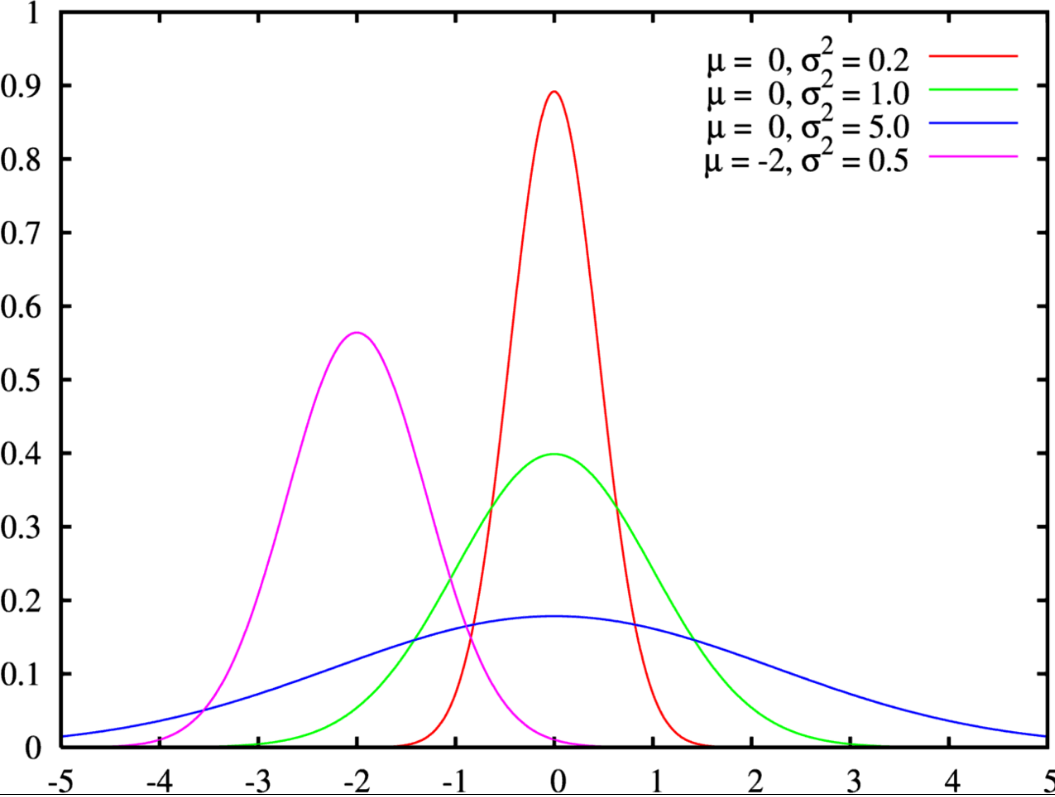
\includegraphics[width=0.7\linewidth]{screenshot001}
	\end{center}
	(imagine preluată de aici: \url{https://ro.wikipedia.org/wiki/Distribu%C8%9Bia_Gauss#/media/Fi%C8%99ier:Normal_distribution_pdf.png})
		
	\textbf{Estimările în sensul verosimilății maxime (MLE) pentru parametrii $\mu$, $\sigma^2$}
	
	Ca de obicei (cum am mai discutat în primele seminarii pentru Bernoulli spre exemplu), în lumea reală parametrii unei distribuții de probabilitate nu sunt cunoscuți. Ceea ce cunoaștem sunt niște date (de exemplu: înălțimile unor oameni), iar din date vom estima parametrii.
	
	Exemplu:
	
	Fie următorul set de date: $D = (1.5,2,3,4,5.5)$. Atunci:
	$$\mu_\text{MLE} = \frac{1.5 + 2 + 3 + 4 +5.5}{5} = 3.2$$
	$$\sigma^2_\text{MLE} = \frac{(1.5 - \mu_\text{MLE})^2 + (2 - \mu_\text{MLE})^2 + (3 - \mu_\text{MLE})^2 + (4 - \mu_\text{MLE})^2 + (5.5 - \mu_\text{MLE})^2}{5} =$$
	$$= \frac{(1.5 - 3.2)^2 + (2 - 3.2)^2 + (3 - 3.2)^2 + (4 - 3.2)^2 + (5.5 - 3.2)^2}{5} = 2.06$$
	
	\subsubsection{Distribuția Normală bivariată}
	Fie $X : \Omega \rightarrow \mathbb{R}^d$. Dacă $X \sim \mathcal{N}(\mu,\Sigma)$ (adică $X$ urmează o distribuție normală/Gaussiană multivariată), atunci $$p(x) = \mathcal{N}(x;\mu,\Sigma) = \frac{1}{(2\pi)^{d/2} \text{det}(\Sigma)^{1/2}} e^{-\frac{1}{2} (x - \mu)^\top \Sigma^{-1} (x - \mu)},$$
	unde $p$ este pdf-ul lui $X$. $X = \begin{bmatrix}
	X_1\\
	\vdots\\
	X_d
	\end{bmatrix} \in \mathbb{R}^{d}$
	
	$\mu =\begin{bmatrix}
	\mu_1\\
	\vdots\\
	\mu_d
	\end{bmatrix} \in \mathbb{R}^{d}$, $\Sigma \in \mathbb{R}^{d \times d}$ sunt parametrii pentru distribuția normală multivariată.
	
	$\mu$ se mai cheamă medie, iar $\Sigma$ se mai cheamă matrice de covarianță. Oare de ce? Pentru că se poate demonstra că $E[X_i] = \mu_i, i\in \{1,\dots,d\}$ și $\text{Cov}(X_i,X_j) = \Sigma_{ij}, \forall i,j \in \{1,\dots,d\}$.
	
	Distribuția normală bivariată este distribuția multivariată atunci când $d = 2$. În acest caz, $\Sigma$ mai este scris astfel:
	$$\Sigma = \begin{bmatrix}
	\sigma_{1}^2 & \sigma_{12}\\
	\sigma_{21} & \sigma_2^2
	\end{bmatrix} = \begin{bmatrix}
	\sigma_{1}^2 & \sigma_{12}\\
	\sigma_{12} & \sigma_2^2
	\end{bmatrix} = \begin{bmatrix}
	\sigma_{1}^2 & \rho \sigma_{1} \sigma_2\\
	\rho \sigma_1 \sigma_2 & \sigma_2^2
	\end{bmatrix},$$
	unde $\rho = \frac{\sigma_{12}}{\sigma_1 \sigma_2}$ este numit coeficientul de corelație.
	
	Pentru cazul bivariat, graficele pentru pdf-ul $p$ în funcție de diferite setări pentru parametrii $\mu$ și $\Sigma$:
	
	\begin{center}
		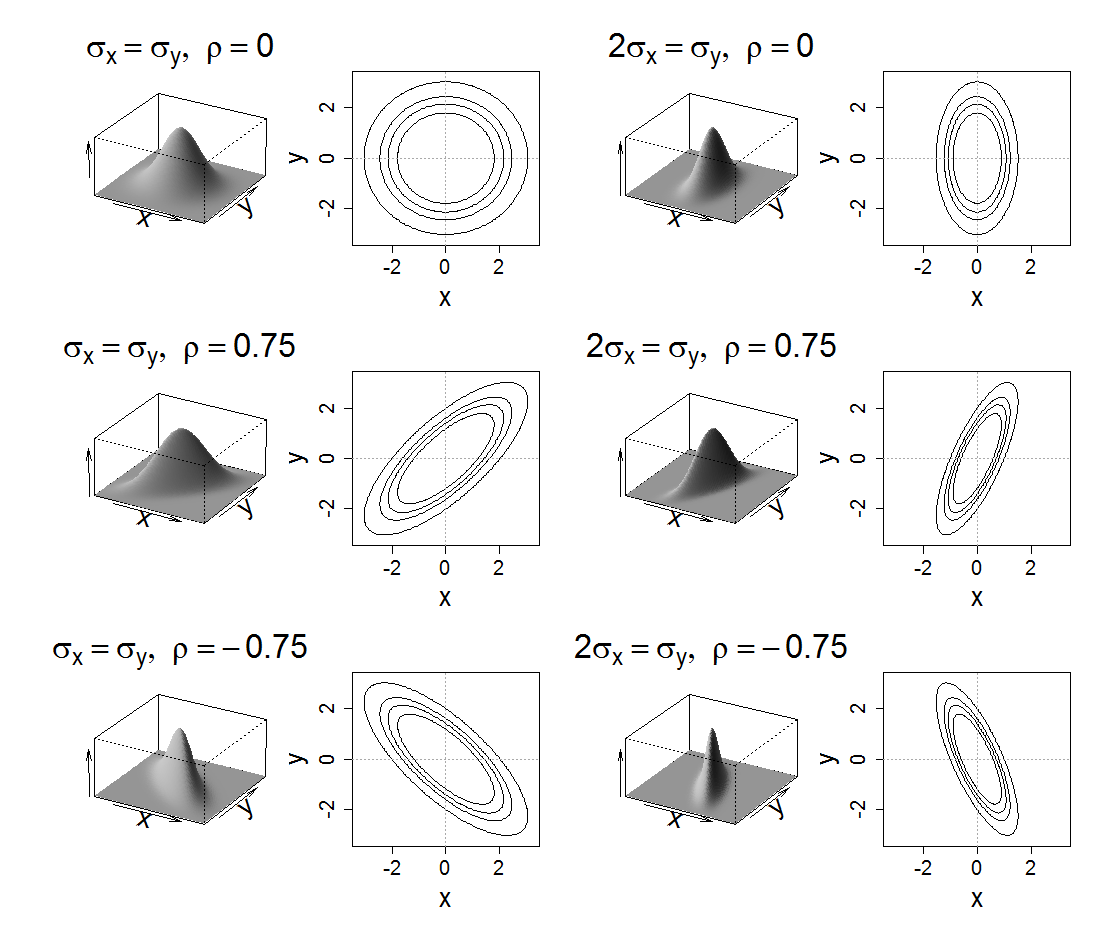
\includegraphics[width=\linewidth]{screenshot002}
	\end{center}
	(imagine preluată de aici: \url{http://www.stat.cmu.edu/~kass/KEB/figures/bivariateNormalRev.png})
	
	Graficele de mai sus în 3D sunt graficele pentru pdf-ul $p$. Graficele în 2D sunt tăieturi ale graficului în 3D cu un plan paralel cu planul de jos (adică Oxy). În exercițiile din carte aveți de-a face cu grafice în 2D. Curbele din graficele 2D se numesc \textit{curbe de izocontur}.
	
	 
	
	\textbf{Proprietate}: Produsul a două pdf-uri ale unor variabile normale univariate independente furnizează un pdf al unei variabile normale bivariate. Urmăriți exemplul:
	
	Dacă $X_1 \sim \mathcal{N}(1,2^2)$ cu pdf-ul $p_1$, $X_2 \sim \mathcal{N}(3,4^2)$ cu pdf-ul $p_2$, atunci pdf-ul $p(x_1,x_2) = p_1(x_1) p_2(x_2)$ corespunde lui $X = \begin{bmatrix}
	X_1\\
	X_2
	\end{bmatrix} \sim \mathcal{N}\left(\begin{bmatrix}
	1\\
	3
	\end{bmatrix}, \begin{bmatrix}
	2^2 & 0 \\
	0 & 4^2
	\end{bmatrix} \right)$.
	
	\textbf{Observație} în legătură cu exemplul anterior: Din matricea $\begin{bmatrix}
	2^2 & 0\\
	0 & 4^2
	\end{bmatrix}$ observăm că $\sigma_{12} = 0 \Rightarrow \rho = 0$. Deci, dacă urmărim și desenul anterior, curbele de izocontur vor semăna cu desenele de pe primul rând (mai mult: vom fi pe cazul coloanei a doua pentru că $\sigma_{X_2} > \sigma_{X_1}$).
	
	\subsection{Extensie Bayes Naiv - atribute continue la intrare}
	
	Vezi ex. 15/pag. 400.
	
	\subsection{Privire de final Bayes Naiv}
	
	În notițele de la semimarul trecut am scris o altă perspectivă asupra alg. NB și JB: \textit{având un rând la testare $(a_1,\dots,a_n)$, gândiți-vă la rândurile $(a_1,\dots,a_n,v_1)$, $(a_1,\dots,a_n,v_2)$, ..., $(a_1,\dots,a_n,v_k)$. Calculați probabilitatea fiecărui rând și returnați eticheta corespunzătoare probabilității maxime.}
	
	Putem să punem acele probabilități într-o sumă astfel:
	
	$$p_\text{NB}(a_1,\dots,a_n) = p_\text{NB}(A_1=a_1,\dots,A_n=a_n) =$$
	$$= p_\text{NB}(A_1=a_1,\dots,A_n=a_n,V=v_1) + \dots + p_\text{NB}(A_1=a_1,\dots,A_n=a_n,V=v_k) = $$
	$$= p_\text{NB}(V=v_1)p_\text{NB}(A_1=a_1|V=v_1)\dots p_\text{NB}(A_n = a_n|V=v_1) + \dots + $$
	$$+ p_\text{NB}(V=v_k)p_\text{NB}(A_1=a_1|V=v_k)\dots p_\text{NB}(A_n = a_n|V=v_k)$$
	
	Astfel, obținem pmf/pdf-ul pentru $(A_1,\dots,A_n)$: $p_\text{NB}(a_1,\dots,a_n)$.
	
	Privirea de final ar fi în felul următor:
	\begin{itemize}
		\item la antrenare: scrieți $p_\text{NB}(a_1,\dots,a_n)$ ca o sumă
		\item la testare: calculați $p_\text{NB}$ pe instanța de test, termen cu termen. Returnați eticheta termenului maxim.
	\end{itemize}
	
	Exemplu:
	
	Fie setul de date următor, unde $X_1$ este discret, iar $X_2$ este continuu:
	
	\begin{center}
		\begin{tabular}{ c|c||c }
			$X_1$ & $X_2$ & Y \\ 
			\hline
			 0& 1 & 0 \\  
			 0& 2 & 0 \\  
 			 1& 3 & 0 \\  
			 0& 4 & 1 \\  
			 1& 5 & 1 \\  
		\end{tabular}
	\end{center}
	
	Antrenare:
	
	$$p_\text{NB}(x_1,x_2) = p_\text{NB}(X_1=x_1,X_2=x_2,Y=0) + p_\text{NB}(X_1=x_1,X_2=x_2,Y=1) = $$
	$$ = p_\text{NB}(Y=0) p_\text{NB}(X_1=x_1|Y=0) p_\text{NB}(X_2=x_2|Y=0) +$$
	$$+ p_\text{NB}(Y=1) p_\text{NB}(X_1=x_1|Y=1) p_\text{NB}(X_2=x_2|Y=1) $$
	$$= \frac{3}{5} \text{Bernoulli}(x_1;\theta=1/3) \mathcal{N}(x_2;\mu=2,\sigma^2=2/3) + $$
	$$ + \frac{2}{5} \text{Bernoulli}(x_1;\theta=1/2) \mathcal{N}(x_2;\mu=4.5,\sigma^2=0.25)$$
	
	Testare: pe instanța $(0,6)$
	
	$$p_\text{NB}(0,6) = \frac{3}{5} \text{Bernoulli}(0;\theta=1/3) \mathcal{N}(6;\mu=2,\sigma^2=2/3) + $$
	$$ + \frac{2}{5} \text{Bernoulli}(0;\theta=1/2) \mathcal{N}(6;\mu=4.5,\sigma^2=0.25)=$$
	$$=0.0000012008 + 0.001772739$$
	
	$0.001772739 > 0.0000012008 \Rightarrow y_{NB} = 1$
	
	\textbf{Observație}: Dacă ambele atribute de intrare erau continue, nu mai înmulțeam Bernoulli cu Normală, ci Normală cu Normală. Ținând cont de această observație și folosind proprietatea și imaginea din \textit{2.3.2 Distribuția Normală bivariată}, puteți înțelege (mai ușor) ex. 16/pag. 402.
	
	Vezi ex. 16/pag. 402.
	
	\newpage
	\textbf{\large{Schemă de final}}
	\begin{enumerate}
		\item Rata medie a erorilor
		\begin{enumerate}
			\item Rata medie a erorilor
			\item Surse de erori pentru NB și JB
		\end{enumerate}
		\item Extensie Bayes Naiv - atribute continue la intrare
		\begin{enumerate}
			\item Remember: Variabile aleatoare discrete
			\begin{enumerate}
				\item Bernoulli, Categorială
				\item MLE pentru Bernoulli, MLE pentru Categorială
			\end{enumerate}
			\item Variabile aleatoare continue
			\begin{enumerate}
				\item Distribuția normală univariată
				\item MLE pentru normală univariată
				\item Distribuțua normală bivariată
				\item Distribuțua normală bivariată - proprietate + desen
			\end{enumerate}
			\item Privire de final Bayes Naiv
		\end{enumerate}
		
	\end{enumerate}
	
\end{document}